Face detection and recognition from video footage have been extensively studied in the field of computer vision and surveillance systems. One of the critical components of this task is the accurate localization and extraction of face regions from individual video frames. Traditionally, this has been achieved through techniques such as Viola-Jones object detection and Histogram of Oriented Gradients (HOG) descriptors. However, recent advancements in deep learning have led to the development of more robust and efficient models for object detection and pose estimation.

\textbf{Pose Estimation and Keypoint Detection using YOLOv8}

You Only Look Once (YOLO) is a state-of-the-art object detection algorithm that has been widely adopted for various computer vision tasks, including pose estimation. The latest version, YOLOv8, introduced by Ultralytics, incorporates advanced techniques for multi-person pose estimation, enabling the localization of up to 17 keypoints on the human body. This capability is particularly relevant for our project, as it allows for the precise extraction of face bounding boxes based on detected facial landmarks.

Pose estimation is a task that involves identifying the location of specific points in an image, usually referred to as keypoints. The keypoints can represent various parts of the object such as joints, landmarks, or other distinctive features. The locations of the keypoints are usually represented as a set of 2D \verb|[x, y]| or 3D \verb|[x, y, visible]| coordinates.

\begin{figure}[H]
    \centering
    \fbox{ 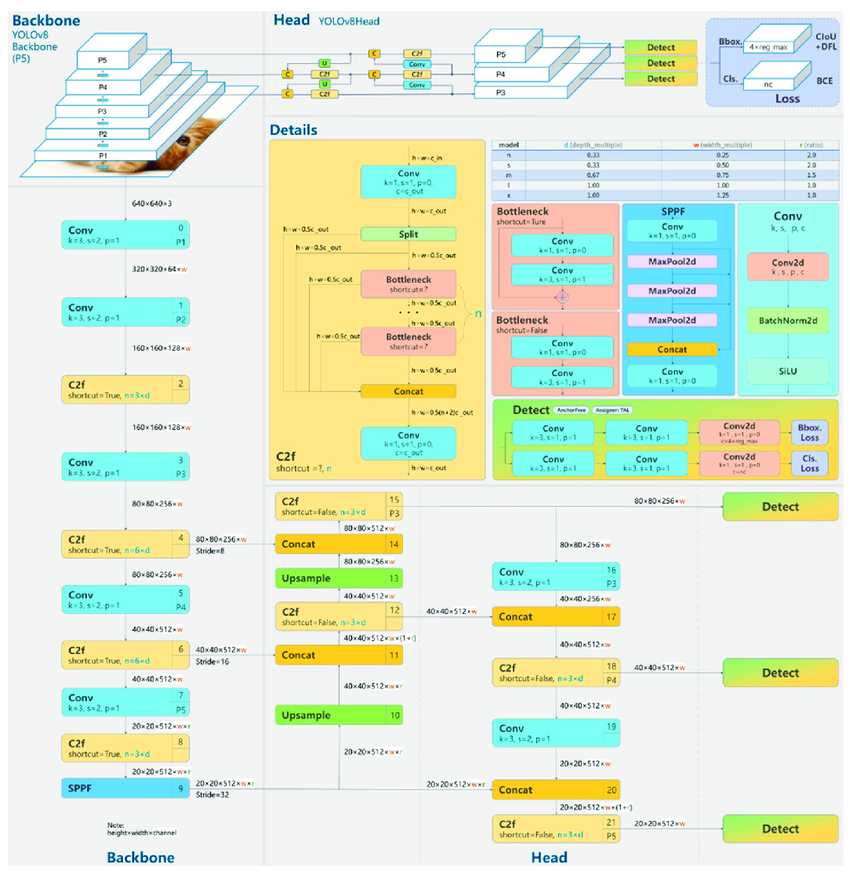
\includegraphics[width=\linewidth]{Yolov8 Architecture.png}}
    \caption{YOLOv8 Architecture}
    \label{fig:enter-label}
\end{figure}

The YOLOv8 pose estimation model is trained on the COCO-Pose dataset, a large-scale object detection, segmentation, and pose estimation dataset derived from the popular COCO dataset. COCO-Pose focuses specifically on human pose estimation and includes multiple keypoints for each human instance. It consists of over 200,000 labeled images, providing a rich and diverse dataset for training robust pose estimation models.

\begin{figure}[H]
    \centering
    \fbox{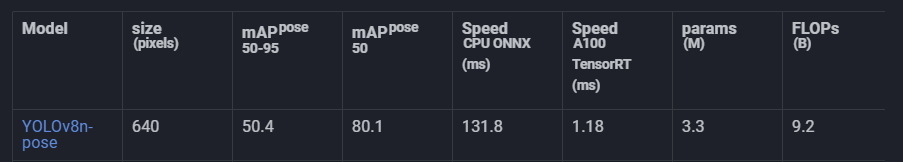
\includegraphics[width=0.9\linewidth]{yolov8 nano pose model.png}}
    \caption{YOLOv8 Pre-trained Nano Pose Detection Model Performance}
    \label{fig:enter-label}
\end{figure}

The output of a pose estimation model is a set of points that represent the keypoints on an object in the image, usually along with the confidence scores for each point. Pose estimation is a good choice when you need to identify specific parts of an object in a scene, and their location in relation to each other.

In addition to COCO-Pose, Ultralytics provides several other datasets for pose estimation tasks, including COCO8-Pose and Tiger-Pose:

\begin{itemize}
    \item \textbf{COCO8-Pose}: A small but versatile pose detection dataset composed of the first 8 images from the COCO train 2017 set, with 4 images for training and 4 for validation. It follows the same label format as COCO-Pose, with 17 keypoints for human poses, and is suitable for testing, debugging, and experimenting with new detection approaches.
    \item \textbf{Tiger-Pose}: An animal pose dataset comprising 263 images sourced from a YouTube video, with 210 images for training and 53 for validation. It follows the Ultralytics YOLO format with 12 keypoints for animal pose and no visible dimension, making it suitable for non-human pose estimation tasks.
\end{itemize}

The COCO-Pose dataset defines 17 keypoints for each human, including the nose, eyes, ears, shoulders, elbows, wrists, hips, knees, and ankles. The model outputs these keypoints in the Ultralytics YOLO format, representing each keypoint as a tuple of (x, y) coordinates and a confidence score for the detection. As a result, our project leverages the YOLOv8 model to accurately localize facial keypoints, which serve as the basis for extracting precise face bounding boxes from video frames.

\pagebreak{}

\textbf{Image Super-Resolution}

While face detection and extraction are crucial steps, the enhancement of low-resolution or poor-quality face images is equally important for effective recognition and identification. Traditional image upsampling techniques, such as bicubic interpolation, often result in blurred or artifact-prone outputs. To address this limitation, deep learning-based super-resolution methods have emerged, leveraging the power of convolutional neural networks (CNNs) and Generative Adversarial Networks (GANs).

The Enhanced Super-Resolution Generative Adversarial Network (ESRGAN), proposed by Wang et al., is a state-of-the-art model for single image super-resolution. It builds upon the seminal work of the Super-Resolution Generative Adversarial Network (SRGAN) and introduces several improvements, including a Residual-in-Residual Dense Block (RRDB) architecture without batch normalization, a relativistic discriminator, and an enhanced perceptual loss function.  Its network architecture is given in the {\textcolor{blue}{Fig 3.}}(\ref{fig:ESRGan}). These advancements enable ESRGAN to generate realistic and natural textures while minimizing artifacts, making it a promising candidate for enhancing the visual quality of face images extracted from video footage.

\begin{figure}[H]
    \centering
    \fbox{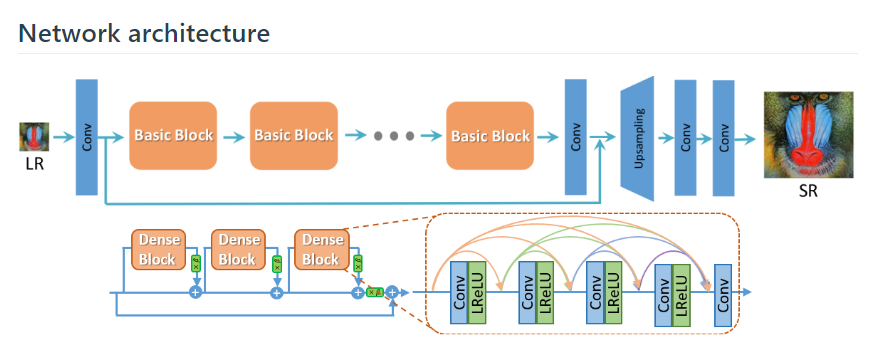
\includegraphics[width=\linewidth]{ESRGAN_network_architecture.png}}
    \caption{Network Architecture of ESRGAN}
    \label{fig:ESRGan}
\end{figure}

ESRGAN has demonstrated superior performance on various benchmarks, such as Set14, BSD-500, and Urban100, outperforming previous state-of-the-art methods. Additionally, it achieved the first place in the PIRM2018-SR Challenge, further validating its effectiveness in the image super-resolution task. 

\begin{figure}[H]
    \centering
    \fbox{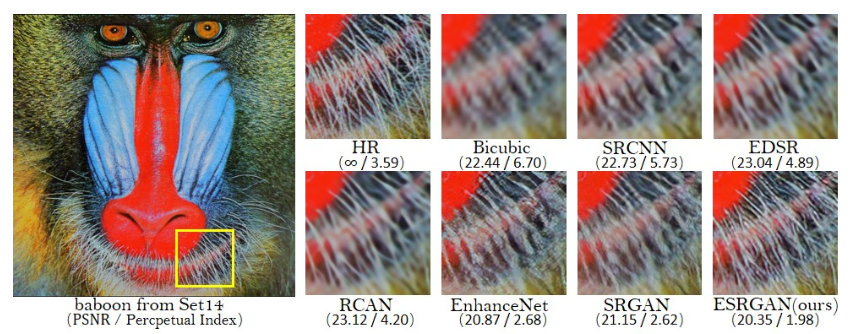
\includegraphics[width=\linewidth]{quantitative results of ESRGan.png}}
    \caption{Quantitative Results - ESRGAN}
    \label{fig:enter-label}
\end{figure}

While existing literature has explored face detection, pose estimation, and image super-resolution individually, our project aims to integrate these components into a comprehensive pipeline tailored for enhancing face images extracted from video surveillance footage. By leveraging the strengths of YOLOv8 for accurate keypoint detection and ESRGAN for high-quality super-resolution, we endeavor to address the challenges posed by low-resolution or poor-quality video data, ultimately improving the effectiveness of surveillance systems for identification and recognition purposes.